\documentclass[a4paper,11pt, oneside]{article}
\usepackage[T1]{fontenc}
\usepackage[utf8]{inputenc}
\usepackage{lmodern}
\usepackage[italian]{babel}
\usepackage[hidelinks]{hyperref}
\usepackage{listings}
\usepackage{dirtree}
\usepackage{float}
\usepackage{listings}
\usepackage{graphicx}
\usepackage{titling}
\usepackage[font=small,labelfont=bf]{caption}
\usepackage{verbatim}
\usepackage{gensymb}

\lstset{
            basicstyle=\ttfamily
        }

\pretitle{%
  \begin{center}
  \LARGE
  
\includegraphics[]{logo_unife}\\[\bigskipamount]
}
\posttitle{\end{center}}

\title{\textbf{UNIVERSITÀ DEGLI STUDI DI FERRARA\\}
\bigskip
Corso di Laurea in Informatica\\
\bigskip
\bigskip
\bigskip
\textit{Ricostruzione tomografica mediante libreria OpenRTK e creazione di un package Python per semplificarne l'utilizzo.\\}
\bigskip
\bigskip
\bigskip
\bigskip
\bigskip
\bigskip
\bigskip
\bigskip
\bigskip
\bigskip
\bigskip
\bigskip
\bigskip
\bigskip
\bigskip
\bigskip
\bigskip
\bigskip
\bigskip
\bigskip
}
\author{Relatore: Giovanni Di Domenico\and
Candidato: Danny Lessio}


\date{Anno Accademico 2015 - 2016}
\begin{document}

    \maketitle
    \newpage
    
    \tableofcontents

    \part{Presentazione}
        \par
            Questa tesi tratta lo studio e l'utilizzo della libreria OpenRTK \cite{openrtk-website} basata su Insight Toolkit (ITK).\cite{itk-website}, la quale fornisce sia un insieme di tools basilari per poter eseguire efficientemente ricostruzioni tomografiche ( filtering, forward projection, backprojection ), sia un set di strumenti per poter eseguire il calcolo a livello multithreaded, sia su CPU che su GPU. Presenta inoltre delle interfacce I/O calibrate per un insieme limitato di CAT scanner attualmente in commercio.
    
        \par
            Per semplificarne l'utilizzo viene realizzato un package Python che si appoggia sia sulla libreria OpenRTK per eseguire le retroproiezioni sia su tools esterni come SimpleITK, una libreria più leggera rispetto ad Insight ToolKit per aiutare nella normalizzazione e conversione delle proiezioni in formato .MHA / .MHD.
            Il package è eseguibile a linea di comando, ed è facilmente estendibile per coprire anche eventuali evoluzioni della libreria OpenRTK.
    
        \par
            [TODO nella sezione X si fa Y etc bla di blabla, il secondo di blabla]
          
        \newpage
        \section{Tomografia Assiale Computerizzata}
            Per tomografia (dal greco \textit{témnó}, tagliare, o \textit{tómos}, nel senso di "strato", e \textit{gráphó}, scrivere) si intende la tecnica spettroscopica mirata alla rappresentazione a strati di un oggetto, in contrapposizione alla radiografia convenzionale la quale dispone sulla superficie bidimensionale della lastra tutto lo spessore del corpo o oggetto.\\
            La tomografia trova impiego soprattutto in medicina, ma anche in archeologia, geofisica, chimica e scienze dei materiali.
            
            \begin{comment}
            <TODO questa parte iniziale non mi piace affattooolooolo>
            infatti puoi inserire una descrizione più dettagliata prelevando la roba da questo libro:
            https://books.google.it/books?id=ba9yAgAAQBAJ&pg=PA202&lpg=PA202&dq=hounsfield+radon&source=bl&ots=rx7UNFYyba&sig=cs2Q6B3sy-LOMMffco3cttyVhxM&hl=it&sa=X&ved=0ahUKEwirqqOKhIrQAhULtBQKHVKsCTAQ6AEIMDAD#v=onepage&q&f=false
            \end{comment}
            
            \subsection{Breve storia}
                \subsubsection{I limiti della radiografia convenzionale}
                    \par
                        Al fine di comprendere l'importanza della Tomografia Computerizzata, è importante comprendere le limitazioni imposte dalla radiografia convenzionale. Questa metodologia è sostanzialmente composta da una sorgente a raggi X, i quali vengono proiettati attraverso il corpo ed impressi su lastra radiografica bidimensionale. E’ essenzialmente il risultato dell’attenuazione media\cite{hounsfield-nobel-lecture} dei raggi dovuta alla composizione del materiale incontrato dalla sorgente alla pellicola. Nel caso in cui l’oggetto in esame sia il corpo umano, la quantità di attenuazione è direttamente proporzionale alla densità dei vari tessuti incontrati: i polmoni, contenendo aria, assorbono poca radiazione; le ossa, essendo molto dense, ne assorbono maggiormente.
                        
                        \begin{figure}[h]
                            \centering
                            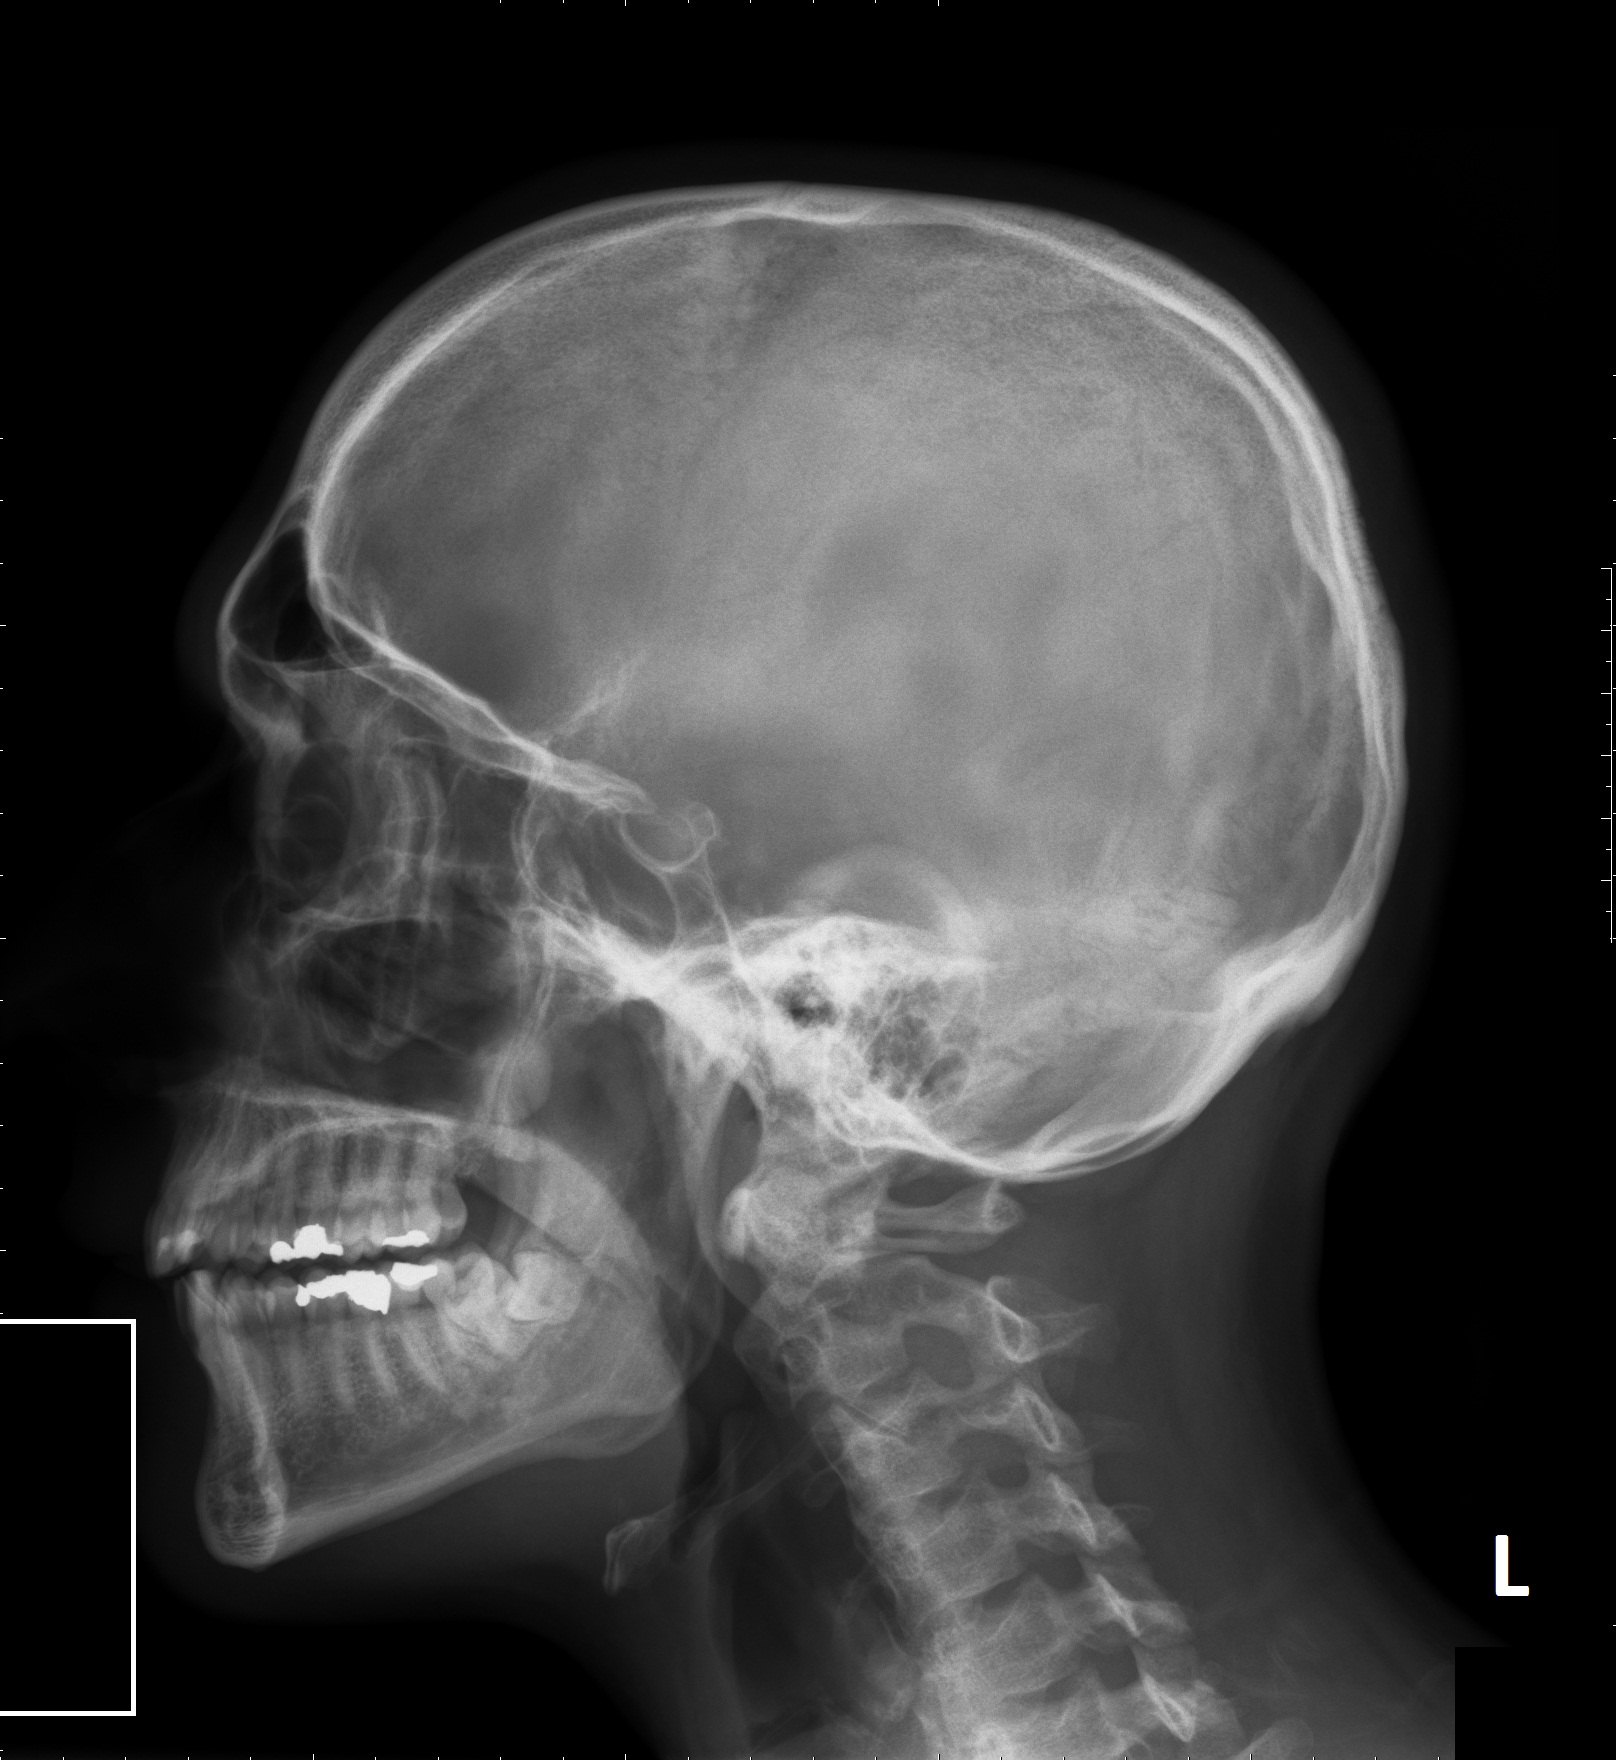
\includegraphics[width=0.4\textwidth]{radiografia}
                            \caption{Una radiografia al cranio - vista laterale.}
                            \label{fig:skull}
                        \end{figure}
                    
                        Dalla radiografia in \texttt{Figura \ref{fig:skull}}, è possibile distinguere solamente cinque vari livelli di densità. Partendo dal meno denso, possiamo visualizzare \textit{l'aria}, di colore nero; \textit{l'acqua o i tessuti molli}, che si visualizzano con un grigio chiaro; \textit{le ossa}, che presentano una colorazione tendente al bianco; \textit{il campione metallico} (L), di colore bianco.
                        \begin{comment}
                            <TODO accertati che sia un campione metallico>
                        \end{comment}
                        L’acqua ed i tessuti molli hanno circa lo stesso livello di attenuazione. Come si sarà notato dalla figura, sarebbe impossibile analizzare il cervello ed evidenziarne una eventuale patologia, poiché esso è rappresentato come una zona omogeneamente grigia. Ottenere un immagine del cervello mediante radiografia classica rimase una sfida sin dal periodo immediatamente successivo al 1985, anno in cui vennero scoperti i raggi X. Anche il grande scienziato ed inventore Thomas Edison agli inizi del '900 si cimentò senza successo nell'impresa, a causa delle grosse limitazioni che l'analisi imponeva.\cite{thomas-edison-brain} Il cervello è infatti composto da tessuti molli, racchiusi all’interno di uno scheletro denso che impedisce alla maggior parte della radiazione di penetrarli, inoltre fluttua a bagno in un liquido chiamato \textit{fluido celebro spinale} il quale fornisce nutrienti ed agisce come cuscino al fine di proteggere la materia grigia stessa. Questo tipo di analisi, si scoprì, essere totalmente inaccessibile alla radiografia convenzionale.
                        
                    \par
                        Un radiogramma impone diversi limiti diagnostici. Il \textit{problema delle ombre} è una diretta conseguenza del fatto che le complesse strutture tridimensionali del corpo umano, nella radiografia, vengono impresse su lastra bidimensionale. Un tumore, ad esempio, se fosse celato da una struttura ad alta densità come le costole, potrebbe passare completamente inosservato alla diagnosi. Questo fu il problema che tormentò i radiologi sin dagli inizi del XX secolo e, come si vedrà nella sezione 1.1.2, fu la ragione che portò allo sviluppo delle prime forme di tomografia classica (non computerizzata).
                        Un altro problema, come accennato precedentemente, deriva dal fatto che la radiografia convenzionale non consente la distinzione tra tessuti molli. Infine, la lastra radiografica risulta un mezzo intrinsecamente inadeguato al fine di registrare le differenze di intensità dovute all'attenuazione dei raggi X durante il passaggio attraverso il corpo.
                    \par
                        Il vero problema della radiografia convenzionale è dunque l'immensa perdita di informazione riscontrata in fase di acquisizione. Il \textit{problema delle ombre} verrà parzialmente risolto con lo sviluppo della tomografia convenzionale, l'analisi dei tessuti molli sarà invece possibile solamente con l'avvento della Tomografia Computerizzata (TC), che consentirà inoltre l'accurata misurazione dei valori d'assorbimento, riuscendo a differenziare la natura del materiale o del tessuto.
                        
                \subsubsection{La tomografia convenzionale}
                    \par
                        Per \textit{tomografia convenzionale} si intende l'ottenimento di un tomogramma senza l'ausilio di computazione. Questa tecnica venne completamente rimpiazzata con la Tomografia Computerizzata intorno al 1980.
                        
                    \par
                        I primi studi risalgono al primo ventennio del 1900 e la tomografia convenzionale, curiosamente, venne indipendentemente scoperta più volte da diversi ricercatori sia Europei che Americani senza che questi condividessero materiale: all'epoca, i livelli di comunicazione non erano affatto sviluppati. Un pensiero espresso da Alessandro Vallebona, uno dei cinque grandi pionieri di questa metodologia, era il seguente: \textit{“quando un settore della scienza e della tecnica è maturo per progredire, per fare un passo avanti, il progresso avviene, a volte contemporaneamente oppure a breve distanza di tempo, promosso da persone diverse, anche in Paesi diversi”}\cite{vallebona-pensiero}.
                        Non è infatti difficile recuperare manoscritti nei quali si rivendicano la paternità dell'opera e violazioni d'utilizzo dei brevetti\cite{vallebona-difesa}. Queste ricerche indipendenti, produssero differenti nomenclature generando molta confusione riguardo l'oggetto di studio. Solamente nel 1962, durante la \textit{International Commission of Radiologic Units and Measurements} (ICRU\footnote{\url{http://www.icru.org/}}), venne selezionata la nomenclatura “tomografia”, che venne presto adottata ovunque nel Mondo.
                        
                    \par
                        Come accennato in sezione 1.1.1, i ricercatori del primo ventennio del ‘900 condivisero uno scopo comune: escogitare un sistema che permettesse la separazione delle ombre registrate quando complesse strutture come il corpo umano venivano impressionate su lastra radiografica. Furono offerte numerose soluzioni ed il metodo più convincente risultò la stratificazione dei tessuti del corpo. In questo modo, utilizzando la geometria proiettiva, il problema delle ombre poteva essere superato, nonostante gli ancora elevati livelli di radiazione richiesti dalla procedura.
                        
                        \begin{figure}[h]
                            \centering
                            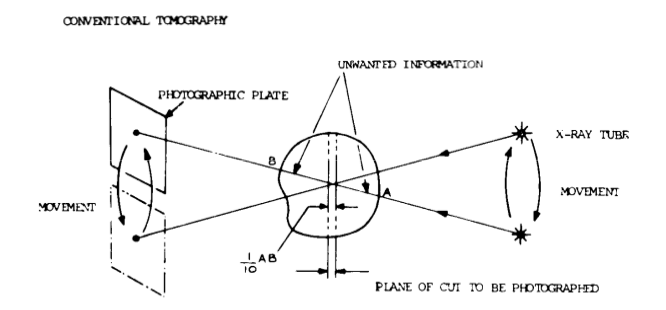
\includegraphics[width=0.8\textwidth]{conventional}
                            \caption{Principio di funzionamento della tomografia convenzionale.}
                            \label{fig:conventional}
                        \end{figure}
                        
                        Per poter eseguire la tomografia convenzionale senza computazione, in un puro sistema meccanico, due dei tre elementi (tubo, paziente e lastra) dovevano necessariamente muoversi in modo sincrono durante l’esposizione alla radiazione.
                        Per poter meglio comprendere il principio di funzionamento, si osservi la \texttt{Figura \ref{fig:conventional}} nella quale si mostra come fosse possibile ottenere una singola slice del corpo basandosi esclusivamente sui principi della geometria proiettiva. In questo caso il corpo (al centro) viene mantenuto fermo, mentre tubo e lastra si muovono in modo sincrono ed opposto. Si può notare che solamente circa 1/10 della lunghezza del fascio AB attraversa effettivamente il piano di interesse; i restanti 9/10 attraversano il corpo collezionando informazione inutile, non voluta. Questa è la motivazione per cui, in questi tomogrammi, era facile riscontrare artefatti\cite{hounsfield-nobel-lecture}.

                    \par
                        André Edmund Marie Bocage, Alessandro Vallebona, Ziedses des Plantes, Gustav Grossmann e Jean Kieffer furono tra i primi ricercatori che contribuirono considerevolmente allo sviluppo di questa nuova metodologia. Bocage nel 1922 ottenne il primo brevetto; Vallebona realizzò diversi prototipi e contribuì alla letteratura con ben 370 pubblicazioni nelle scienze radiologiche\cite{vallebona-ricordo}; des Plantes è ritenuto il pioniere della sperimentazione; Grossmann contribuì all’analisi matematica del metodo e rese più snelli i progetti preesistenti; Kieffer fu il primo pioniere Americano, diede una descrizione esaustiva del suo dispositivo e alla matematica del sistema. I prototipi creati da questi pionieri vennero per lo più utilizzati a scopi di ricerca, l'utilizzo, se a fine clinico, non era affatto confortevole.

                    \par
                        Lo sviluppo del primo dispositivo clinico per la tomografia convenzionale, il Polytome, venne sviluppato a Parigi nel 1950. Le immagini ricavate da questo dispositivo stimolarono le ricerche in ambito clinico, inizialmente dagli Europei e successivamente dagli Americani (anni ‘60).
                        
                        \begin{figure}[h]
                            \centering
                            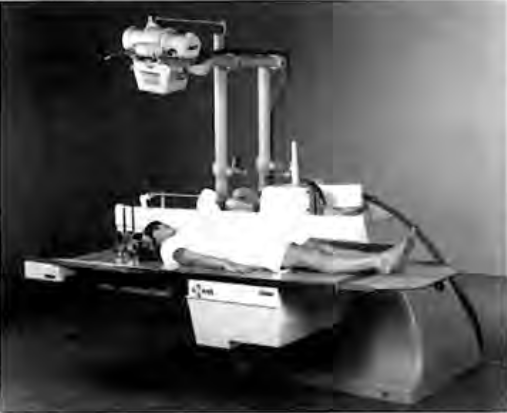
\includegraphics[width=0.5\textwidth]{polytome}
                            \caption{L'Universal Polytome, sviluppato a Parigi dalla Massiot-Philips.}
                            \label{fig:polytome}
                        \end{figure}
                    
                        
                        Le applicazioni più frequenti, riguardavano quelle parti del corpo in cui poteva essere presente un alto livello di contrasto, come il cranio. Queste immagini sezionali permettevano l’esplorazione dell’intricata rete ossea, tra cui i seni paranasali, la sella turcica\footnote{La sella turcica o sella turca costituisce la faccia superiore del corpo dell'osso sfenoide, un osso impari e mediano del neurocranio.} ed altre aree completamente inaccessibili alla radiografia convenzionale. Comparirono successivamente al Polytome diversi nuovi dispositivi che evidenziarono la necessità di ottenere un efficace imaging sezionale.
                    \par
                        E’ importante notare che la tomografia convenzionale non permise l’accesso all’imaging dei tessuti molli, un’immagine sezionale del cervello risulterà quindi possibile solo con l’avvento della Tomografia Computerizzata. Si può storicamente affermare che la tomografia convenzionale ha gettato le basi al di sopra delle quali si sono evolute le avanzate tecnologie di imaging sezionale computerizzato che oggi apprezziamo.
                    
                \subsubsection{Nascita della Tomografia Computerizzata}
                    \par
                        
                        La nascita della Tomografia Computerizzata riflette l'evoluzione della tomografia classica. Il pensiero di Vallebona, citato nella sezione 1.1.2, ha validità anche in questo caso: tre ricercatori, Allan McLeod Cormack, William H. Oldendorf e Godfrey N. Hounsfield, indipendentemente, svilupparono i principi base della TC intorno al 1960. Cormack ed Hounsfield ricevettero il Premio Nobel nel 1979, Oldendorf fu invece vittima di una controversia\cite{nobel-debate} e non venne premiato. 
                        Sia Cormack che Oldendorf ottennero prototipi funzionanti, ma l'ingegnere britannico Godfrey N. Hounsfield fu l'unico in grado di ottenere diverse realizzazioni commerciali di successo.
                    \par
                        Hounsfield lavorò dal 1951 per la EMI Ltd di Londra, periodo nel quale si interessò particolarmente ai computer e contribuì alla costruzione del primo computer a transistor in assoluto assemblato in Gran Bretagna\cite{housfield-autobiografia}. Successivamente, negli anni '60, egli concepì l’idea della Tomografia Computerizzata ed iniziò le prime sperimentazioni.
                        
                        \begin{figure}[h]
                            \centering
                            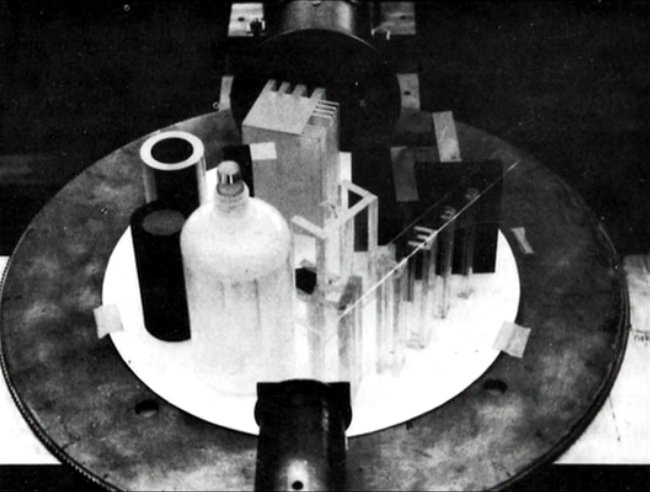
\includegraphics[width=0.5\textwidth]{first-prototype}
                            \caption{Il primo prototipo realizzato da Hounsfield}
                            \label{fig:prototype}
                        \end{figure}
                        
                        Il primo prototipo era composto da una scatola di piombo con un piccolo foro posto nella parte anteriore, all’interno della quale era presente un materiale radioattivo, l’Americium, capace di fornire una fonte costante, non particolarmente intensa, di raggi gamma. La radiazione fuoriusciva dal foro in singolo fascio collimato a configurazione pencil-beam. Il piatto visibile in \texttt{Figura \ref{fig:prototype}} veniva traslato orizzontalmente per permettere al singolo fascio di poter raggiungere tutti gli oggetti. Al termine della traslazione, il piatto veniva fatto roteare di un grado, ed il procedimento veniva ripetuto. I livelli d'attenuazione erano letti dai detector opposti alla sorgente. Il processo di scansione durò ben nove giorni, la ricostruzione\footnote{<TODO verrà trattata laggiu>} computerizzata degli oggetti richiese più di due ore di processamento. Questo fu un risultato molto importante, poiché dimostrò che la Tomografia Computerizzata era tecnologicamente e fisicamente possibile.
                       
                        Hounsfield ed i suoi collaboratori, mantenendo la stessa geometria a rotazione-traslazione, continuarono lo sviluppo dei prototipi diminuendo sempre più il tempo di acquisizione. Si resero presto conto che l'avanzamento tecnologico avrebbe permesso l'analisi dei tessuti molli, ma non furono ancora certi che questo avrebbe permesso la localizzazione spaziale dei tumori. A verifica di ciò venne creato il primo dispositivo ad utilizzo clinico, molto più veloce e sofisticato rispetto ai prototipi precedenti, dedicato alla sola analisi del cranio, che doveva rimanere estremamente fermo durante la scansione.
                        
                        \begin{figure}[h]
                            \centering
                            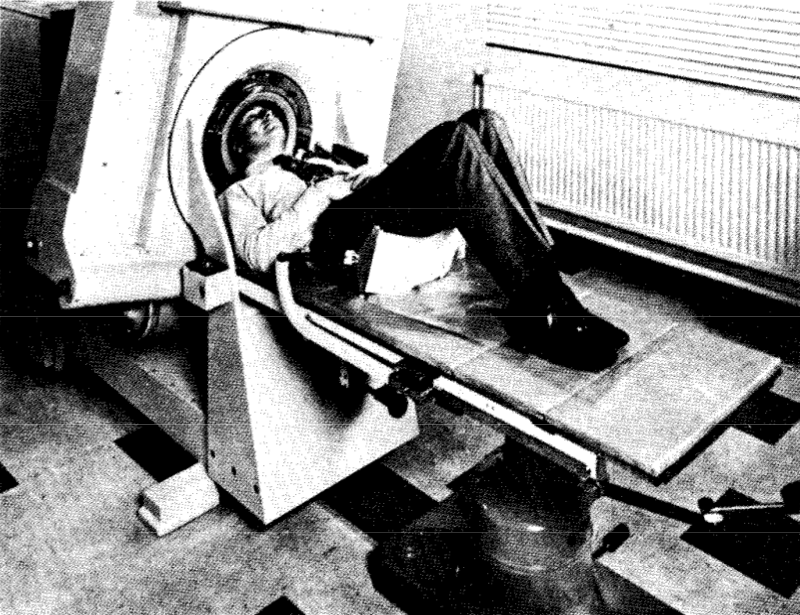
\includegraphics[width=0.5\textwidth]{clinical}
                            \caption{Il primo dispositivo ad utilizzo clinico installato all'Atkinson Morley’s Hospital di Londra.}
                            \label{fig:clinical}
                        \end{figure}
                        
                        Nel 1972 la prima paziente in assoluto fu una donna, il cui cervello si pensava presentasse anomalie. La prima immagine clinica ottenuta con il dispositivo in \texttt{Figura \ref{fig:clinical}} rivelò in chiaro ed inconfondibile dettaglio una cisti circolare nera situata nel lobo frontale della paziente, che fu successivamente operata con successo. Furono analizzati molti altri pazienti, e diventò palese che la macchina risultava perfettamente in grado di effettuare con accuratezza sia l'analisi dei tessuti molli sia la distinzione tra tessuti sani e malati\cite{hounsfield-nobel-lecture}.
                        Per la prima volta nella storia, i limiti imposti dalla radiografia convenzionale visti in sezione 1.1.1 risultarono completamente superati e si aprì la strada ad una rapida innovazione che coinvolse la riduzione dei tempi di esposizione e l'analisi di tutte le parti del corpo. Il team coordinato da Hounsfield già qualche anno dopo, riuscì a costruire macchinari sempre più complessi, con un tempo di acquisizione prossimo ai tre secondi.
                        
                \subsubsection{Evoluzione generazionale CT}
                    \par
                        Per evoluzione generazionale si intende la sequenza temporale nel quale un particolare tipo di CT scanner, avente una ben precisa disposizione dei componenti e specifiche caratteristiche nei movimenti meccanici di base, è stato introdotto nel mercato. E’ importante notare, che al crescere del numero di generazione non crescono necessariamente le performance del sistema.
                    
                    \bigskip
                    \par
                        \textbf{Scanner di prima generazione.} Lo scanner riportato in figura XXX appartiene alla prima generazione. La sorgente veniva collimata in un raggio pencil-beam direzionato ad un singolo detector allineato alla sorgente era posizionato all’altro lato del paziente. Una singola proiezione veniva ottenuta muovendo il tubo sorgente ed il detector in una traslazione. Per poter ottenere la successiva proiezione, l’intera struttura ruotava di 1\degree e veniva traslata nella direzione opposta. Questo processo, di rotazione e traslazione, doveva essere ripetuto fino all’ottenimento di 180 proiezioni. Le prime versioni richiedevano circa 4.5 minuti per poter portare a termine la scansione, ed erano limitate a quelle parti del corpo dove il movimento del paziente poteva essere controllato (testa). Le immagini presentavano una risoluzione bassa.
                        
                        \begin{figure}[h]
                            \centering
                            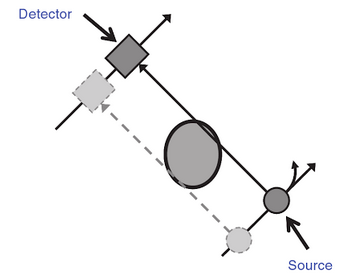
\includegraphics[width=0.4\textwidth]{first-generation}
                            \caption{Rappresentazione schematica di uno scanner di prima generazione.}
                            \label{fig:third-generation}
                        \end{figure}
                        
                    \bigskip
                    \par
                        \textbf{Scanner di seconda generazione.} Il maggiore sforzo per il miglioramento fu concentrato nella riduzione dei tempi di acquisizione, fino al punto di poter ottenere l’imaging di sezioni come il tronco. Aggiungendo detectors disposti angolarmente, diverse proiezioni potevano essere ottenute in una singola traslazione. Una delle prime applicazioni, ad esempo, che presentava 3 detectors con displacement di 1\degree, poteva effettuare 60 traslazioni anzichè 180. Questo era dovuto al fatto che ciascun detector vedeva la sorgente ad un angolo differente, ottenendo in una singola traslazione ben 3 proiezioni. Il sistema, una volta terminata la traslazione, poteva roteare di 3° ed ottenere la nuova proiezione. I tempi di scansione erano quindi ridotti di un terzo. 
                    
                    \bigskip
                    \par
                        \textbf{Scanner di terza generazione.} In questi scanner, la sorgente è collimata in una struttura a ventaglio (fan-beam) diretta verso i detector disposti ad arco. Durante la scansione, il tubo e l’array di detector ruotano lungo il paziente e differenti proiezioni sono attenute durante la rotazione facendo pulsare la sorgente a raggi X o campionando i detector ad un elevato rate. Il sistema puramente rotazionale ha permesso l’accesso a sorgenti a più elevata potenza, permettendo una notevole riduzione dei tempi d’acquisizione. Un aspetto di questa geometria è che i raggi in una singola proiezione sono divergenti anziché paralleli. La divergenza dei raggi richiede qualche modifica all’interno degli algoritmi di ricostruzione. Tutti gli scanner CT odierni sono basati su modifiche di questo design. I tempi di acquisizione sono dell’ordine di pochi secondi e le recenti versioni riescono a scendere sotto al secondo.
                        
                        \begin{figure}[h]
                            \centering
                            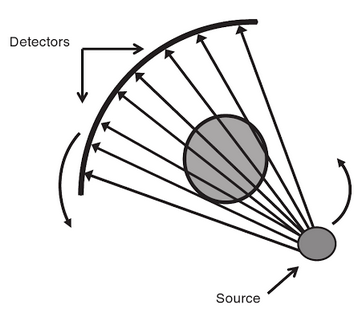
\includegraphics[width=0.5\textwidth]{third-generation}
                            \caption{Rappresentazione schematica di uno scanner di terza generazione.}
                            \label{fig:third-generation}
                        \end{figure}

                    \bigskip
                    \par
                        \textbf{Scanner di quarta generazione.} Questo particolare design si evolse simultaneamente alla terza generazione. In questo particolare caso, viene fatta roteare solo la sorgente e si ha un intero anello composto da detector. Inizialmente questi dispositivi avevano 600 detector, successivamente arrivarono fino a 4800, con tempi di acquisizione comparabili agli scanner di terza generazione. Questo design ha presentato diverse limitazioni, una è dovuta all’ inefficiente utilizzo dei detector (meno di ¼ è effettivamente utilizzato ad ogni istante della scansione) e l’altra è dovuta ad una maggior suscettibilità alla presenza di artefatti (dovuti allo scattering). Per queste ragioni questi scanner non sono più commercialmente disponibili. Una limitazione di questa tipologia di design è la minor efficienza nell’utilizzo dei detector solo meno di ¼ è effettivamente utilizzato ad ogni punto durante la scansione. 
                        
                    \bigskip
                    \par
                        \textbf{Scanner ad elica.} La tecnica coinvolge la continua acquisizione di proiezioni attraverso l’intero volume del paziente. La procedura viene eseguita roteando continuamente la sorgente ed i detector accompagnando il movimento del paziente in una traslazione all’interno del gantry\footnote{TODO footnote gantry}. Per poter ottenere un applicazione funzionante di questo tipo sono necessarie tre tecnologie: la \textit{Slip-Ring Technology}\footnote{Architettura composta da anelli conduttivi elettromeccanici che permettono al frame di scansione di poter roteare continuamente, senza doversi preoccupare dei cavi.}, tubi a raggi X ad elevata energia ed algoritmi di interpolazione che gestiscano le proiezioni non complanari. E’ una tecnologia molto importante perchè per la prima volta nella storia permette la scansione dell’intero corpo del paziente in tempi brevissimi.

                        \begin{figure}[h]
                            \centering
                            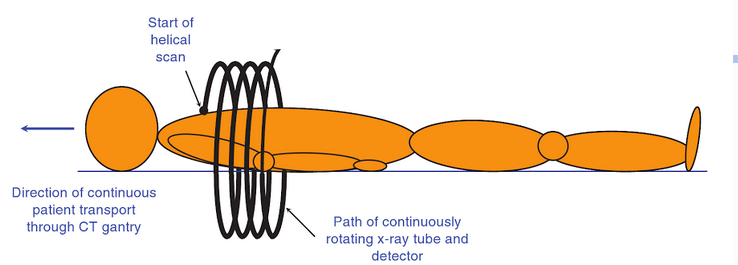
\includegraphics[width=0.5\textwidth]{helix}
                            \caption{Rappresentazione schematica di uno scanner ad elica.}
                            \label{fig:helix}
                        \end{figure}

            
            \subsection{Architetture}
                \subsubsection{Cone Beam}
                \subsubsection{A Spirale}
                \subsubsection{Ad Emissione}
            
            \subsection{Principi di funzionamento}
                \subsubsection{Qualche semplice esempio}
                \begin{comment}
                    potresti parlare della macchina da corsa, vista frontale, laterale, posteriore etc.
                \end{comment}
                \subsubsection{Proiezione - Trasformata di Radon}
                \subsubsection{Filtering}
                \subsubsection{Ricostruzione - Antitrasformata di Radon}
                    In questa sezione puoi pigliare l'introduzione di questo libro:
                    \url{https://books.google.it/books?id=pqSNAgAAQBAJ&pg=PA35&lpg=PA35&dq=%22radiant+energy+apparatus+for+investigating+selected+areas+of+interior+objects+obscured+by+dense+material&source=bl&ots=tvcx6PeTbo&sig=IjYEBPukA9hr7Wrt9RTAekVzbjU&hl=it&sa=X&ved=0ahUKEwiS3JuF4Y7QAhUKbhQKHSMKCUoQ6AEIKjAD#v=onepage&q=%22radiant%20energy%20apparatus%20for%20investigating%20selected%20areas%20of%20interior%20objects%20obscured%20by%20dense%20material&f=false}
                \subsubsection{Retroproiezione}
            
               
                        
    \part{Librerie Utilizzate}
        \section{OpenRTK}
            \subsection{Storia del progetto}
                \par 
                    Il progetto nacque nel Giugno 2010 quando i founder Simon Rit e Gregory Sharp discussero riguardo la scarsità di soluzioni open-source nell'ambito della Cone-Beam CT. Infatti, l'unica alternativa presente era una libreria chiamata Plastimatch, la quale poteva già effettuare retroproiezioni filtrate sia su CPU che su GPU, ma l'architettura del software non teneva conto dell'evoluzione verso nuove tipologie di algoritmi iterativi. Decidettero quindi di dar vita ad una nuova piattaforma basata su Insight ToolKit (ITK), una libreria di elaborazione delle immagini già famosa all'epoca.
                \par
                    Attualmente ( Agosto 2016 ) il Progetto viene mantenuto e sviluppato sulla piattaforma GitHub, ha circa 4000 commit e 20 sviluppatori attivi.
            \subsection{Geometria}
            \subsection{Formato Immagini}
                \subsubsection{.mha}
                \subsubsection{.mhd}
            
            
        \section{SimpleITK}
            \subsection{Storia del progetto}
        
    \part{Lavoro Svolto}
        \section{Compilazione OpenRTK}
            \subsection{Abilitazione Wrapping}
        \section{Compilazione SimpleITK}
            \subsection{Abilitazione Wrapping}
        \section{RTK-Handler}
            \subsection{Scopo}
            \subsection{Architettura}
            \subsection{Utilizzo}
            \subsection{Estensione}
            \subsection{Utilizzi futuri}
            
    \part{Risultati e Conclusioni}
        \subsection{Risultati}
        \subsection{Conclusioni}



\newpage
\begin{thebibliography}{1}
    \bibitem{zeng-tomos}
        Gengsheng, Z. L. (2010). Basic Principles of Tomography. In Springer (Ed.), \textit{Medical Image Reconstruction: A Conceptual Tutorial}.
        
    \bibitem{openrtk-website}
        \url{http://www.openrtk.org/}
    
    \bibitem{itk-website}
        \url{https://itk.org/}
    
    \bibitem{conventional-tomography}
        Littleton, J.T. "Conventional Tomography". A History of the Radiological Sciences (PDF). American Roentgen Ray Society. Retrieved 11 January 2014.
    
    \bibitem{vallebona-ricordo}
        Franco Bistolfi, Alessandro Vallebona 1899-1987. Ricordo di un grande radiologo e del suo contributo allo sviluppo delle scienze radiologiche (PDF), in Fisica in Medicina, nº 2, 2005, pp. 115-123.
        
    \bibitem{vallebona-pensiero}
        Vallebona A. - Gli ottanta anni della radiologia medica in Liguria. Atti dell’Accademia Ligure di Scienze e Lettere, XXXI: 18-46,1974
        
    \bibitem{thomas-edison-brain}
        \url{https://www.researchgate.net/publication/18576763_Thomas_Edison's_attempts_at_radiography_of_the_brain_1896}
        
    \bibitem{hounsfield-nobel-lecture}
        Godfrey N. Hounsfield - Nobel Lecture, 8 December 1979
        
    \bibitem{vallebona-difesa}
        \url{http://www.fisicamedica.it/museo_virtuale/02_sezioni/articoli/data/Vallebona%20difesa.pdf}
        
    \bibitem{nobel-debate}
        Riddle of the Nobel debate - Science 04 Jan 1980: Vol. 207, Issue 4426, pp. 37-38
        
    \bibitem{hounsfield-autobiografia}
        \url{https://www.nobelprize.org/nobel_prizes/medicine/laureates/1979/hounsfield-bio.html}
        
        
    \end{thebibliography}
\end{document}
